% Overleaf instructions:
% 1. Create a new blank project and copy this file into main.tex.
% 2. Create a folder named "figures" and upload the following two files:
%    - section9_cumulative_return_means_only.png
%    - section9_max_drawdown_comparison.png
% 3. Compile with pdfLaTeX. If the figures are absent, labelled placeholders are
%    shown so that the source remains compilable.

\documentclass[10pt,a4paper,BCOR=8mm,headinclude=false,footinclude=false]{scrartcl}

\usepackage[british]{babel}
\usepackage[utf8]{inputenc}
\usepackage[T1]{fontenc}
\usepackage{newpxtext,newpxmath}
\usepackage{amsmath,amssymb,bm}
\usepackage{booktabs,tabularx}
\usepackage{graphicx}
\usepackage{caption}
\usepackage{microtype}
\usepackage{sectsty}
\usepackage{fancyhdr}
\usepackage{lastpage}
\usepackage[hidelinks]{hyperref}
\usepackage{xcolor}

\setlength{\textheight}{250mm}
\setlength{\textwidth}{175mm}
\setlength{\hoffset}{-25mm}
\setlength{\voffset}{-15mm}
\setlength{\parindent}{0pt}
\setlength{\parskip}{0.42em}
\setlength{\abovedisplayskip}{0.45em}
\setlength{\belowdisplayskip}{0.45em}
\setlength{\textfloatsep}{0.7em}
\setlength{\intextsep}{0.6em}
\renewcommand{\arraystretch}{1.08}
\allsectionsfont{\normalfont\scshape}
\sectionfont{\centering\normalfont\scshape\large}
\subsectionfont{\normalfont\scshape\normalsize}
\captionsetup{font=small,labelfont=bf,skip=3pt}

\fancypagestyle{plain}{%
  \fancyhf{}
  \renewcommand{\headrulewidth}{0pt}
  \renewcommand{\footrulewidth}{0.4pt}
  \fancyfoot[L]{\textit{\footnotesize ECE2500Y}}
  \fancyfoot[C]{\textit{\footnotesize Housen Zhu}}
  \fancyfoot[R]{\textit{\footnotesize Page \thepage\ of \pageref*{LastPage}}}
}
\pagestyle{plain}

% Prefer the compact Overleaf paths. The repository paths are fallbacks for a
% local compilation from reports/. The final branch displays a placeholder.
\newcommand{\returnfigure}{%
  \IfFileExists{figures/section9_cumulative_return_means_only.png}{%
    \includegraphics[width=\linewidth]{figures/section9_cumulative_return_means_only.png}%
  }{\IfFileExists{../evaluation/section9_simplex_v3.2_policy_comparison/section9_cumulative_return_means_only.png}{%
    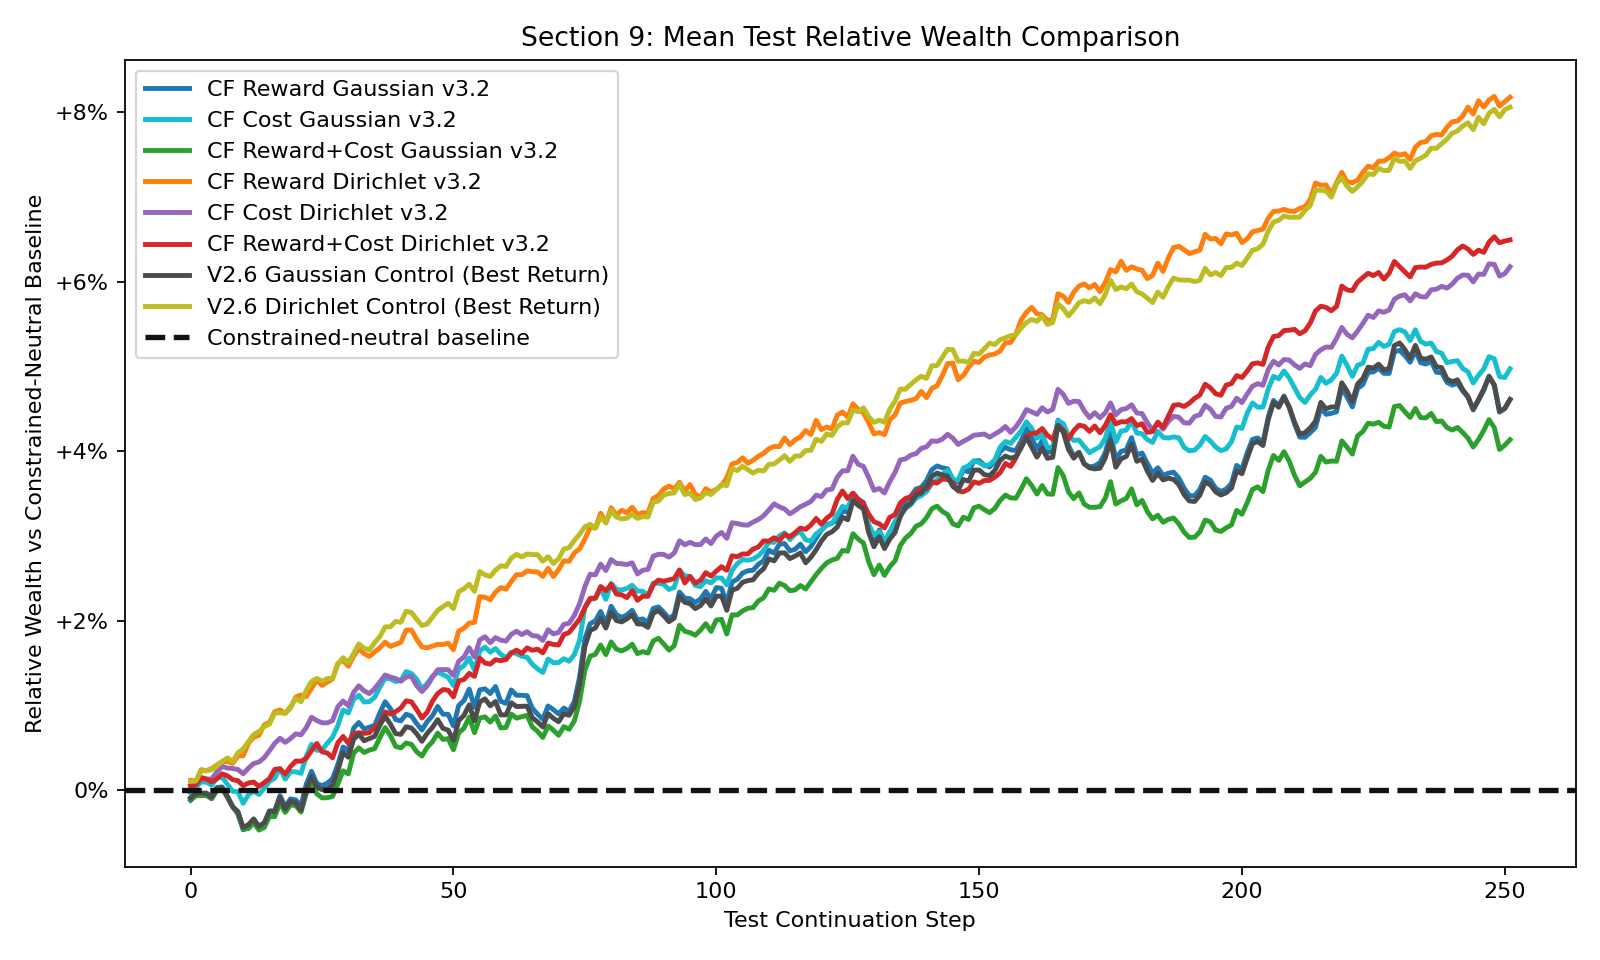
\includegraphics[width=\linewidth]{../evaluation/section9_simplex_v3.2_policy_comparison/section9_cumulative_return_means_only.png}%
  }{\fbox{\parbox[c][42mm][c]{0.96\linewidth}{\centering\small Missing figure\\Upload the cumulative-return PNG to \texttt{figures/}.}}}}%
}
\newcommand{\riskfigure}{%
  \IfFileExists{figures/section9_max_drawdown_comparison.png}{%
    \includegraphics[width=\linewidth]{figures/section9_max_drawdown_comparison.png}%
  }{\IfFileExists{../evaluation/section9_simplex_v3.2_policy_comparison/section9_max_drawdown_comparison.png}{%
    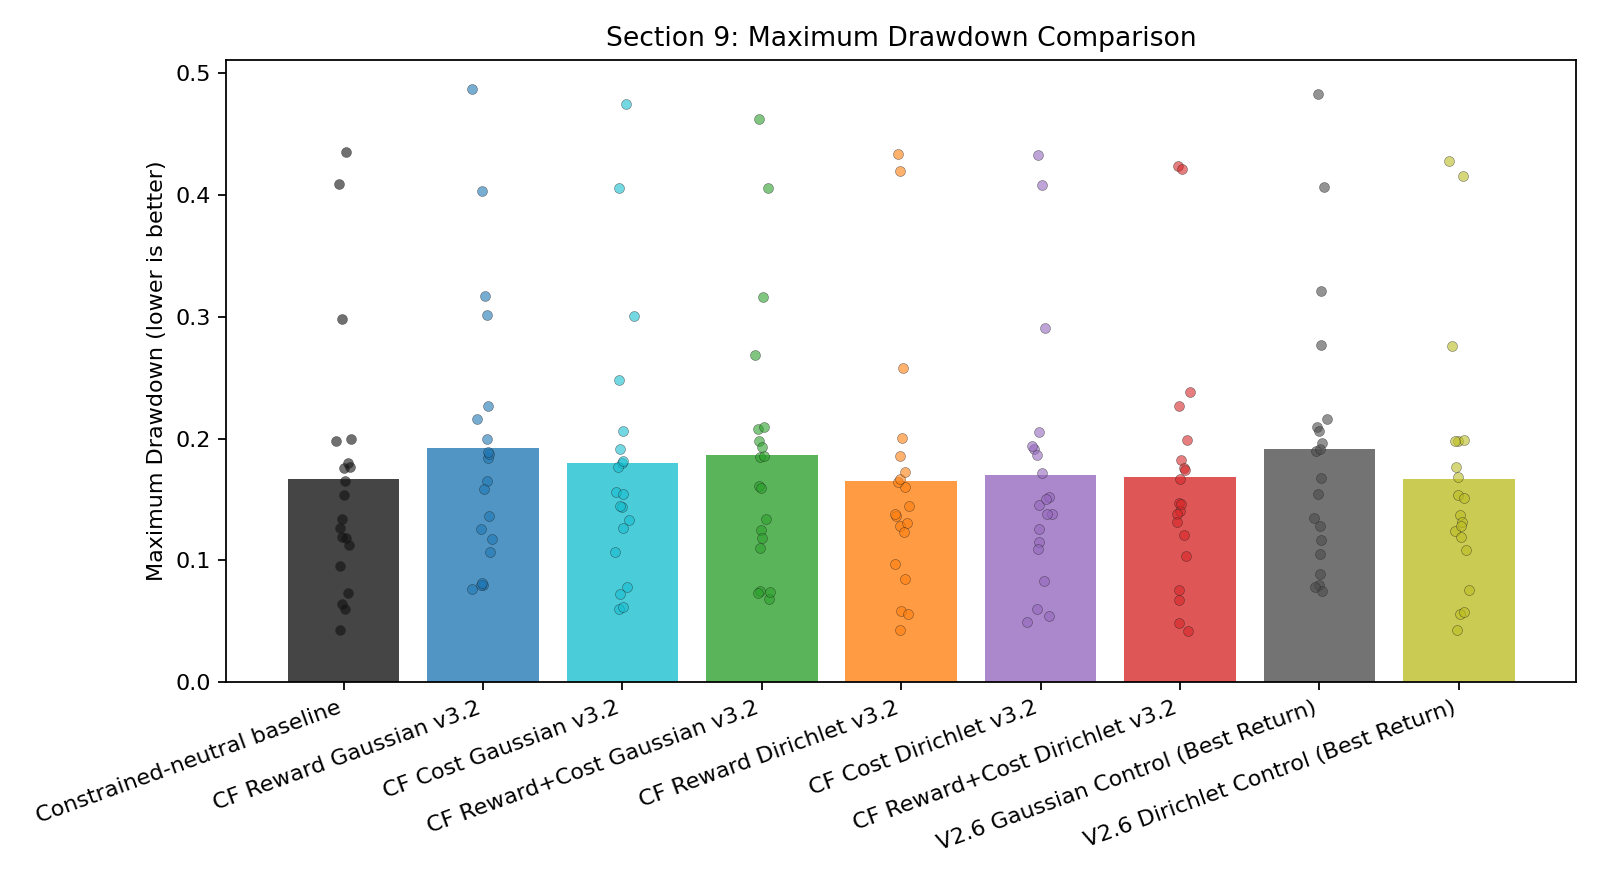
\includegraphics[width=\linewidth]{../evaluation/section9_simplex_v3.2_policy_comparison/section9_max_drawdown_comparison.png}%
  }{\fbox{\parbox[c][42mm][c]{0.96\linewidth}{\centering\small Missing figure\\Upload the maximum-drawdown PNG to \texttt{figures/}.}}}}%
}

\newcommand{\R}{\mathbb{R}}
\newcommand{\simplex}{\Delta^{N}}
\newcommand{\CAOSD}{\operatorname{CAOSD}}

\begin{document}

\begin{center}
  \rule{\linewidth}{0.5pt}\\[-0.1em]
  \small University of Toronto \textbar{} Department of Electrical and Computer Engineering\\
  ECE2500Y: MEng Research Project \hfill Supervisor: A. Bereyhi\\[-0.15em]
  \rule{\linewidth}{0.5pt}\\[0.7em]
  {\LARGE\bfseries Towards Robust Portfolio Reinforcement Learning with\\[0.12em]
  Constraint-Aware Simplex Decomposition\par}
  \vspace{0.45em}
  {\large Housen Zhu}\qquad
  {\small 10 September 2026}
\end{center}
\vspace{-0.5em}

\begin{abstract}
This report studies portfolio reinforcement learning (RL) when static allocation requirements and path-dependent risk limits must be treated differently. We combine Constrained Allocation Optimization with Simplex Decomposition (CAOSD) with Reward Constrained Policy Optimization (RCPO). CAOSD maps autoregressive Gaussian-logit or Dirichlet branch actions into long-only portfolios that satisfy two overlapping minimum-exposure constraints at every decision. RCPO separately penalises benchmark-relative current-drawdown violations through a global Lagrange multiplier. To address interacting branch actions, we evaluate an open-loop counterfactual credit rule that replaces one realised branch by a neutral action while holding the remaining realised branches fixed. Policies receive the same 60,000-update interaction budget on eight synthetic regime-switching markets and are evaluated deterministically on 20 unseen one-year continuations. Counterfactual-reward Dirichlet RCPO has the highest observed mean terminal relative wealth, $8.18\%$, but exceeds its standalone-credit control by only $0.12$ percentage points and requires materially higher turnover. By contrast, counterfactual-cost Gaussian RCPO produces the clearest drawdown improvement over its matched control, again with higher turnover. Joint counterfactual reward and cost is not consistently beneficial. Allocation feasibility is guaranteed by construction; reliable out-of-sample drawdown feasibility is not. Claims are therefore limited to single-seed synthetic experiments.
\end{abstract}

\section{Introduction and Contributions}

Portfolio selection is a sequential control problem: each allocation determines immediate return, transaction costs, and the wealth state from which later decisions are made. Deep RL can represent such feedback, but an unconstrained return objective does not encode institutional allocation mandates or path-risk preferences. The two requirements are mathematically distinct. Long-only and minimum-exposure rules define a static feasible polytope and should hold for every action. Drawdown, by contrast, depends on the realised wealth path and cannot be enforced by projecting a single action.

Prior portfolio RL studies illustrate the flexibility of sequential allocation while repeatedly identifying transaction costs, constraint handling, and out-of-sample stability as central difficulties \cite{gollart2025}. Safe RL casts such requirements as constrained Markov decision processes (CMDPs) \cite{kushwaha2025}. Reward Constrained Policy Optimization (RCPO) adapts a Lagrange multiplier from observed constraint cost \cite{tessler2019}, whereas CAOSD represents a linearly constrained allocation region by coupled simplex subproblems \cite{winkel2023}. Their combination yields a useful division of labour: geometry enforces action-level feasibility, while optimisation expresses a preference over path-dependent risk within that feasible set.

This distinction also clarifies why a single penalty mechanism is insufficient. An expected allocation penalty can make violations rare without ruling them out on a particular rebalance, and a post-hoc projection can distort the action whose probability was evaluated by the policy gradient. Conversely, a static feasible-set map cannot determine whether a sequence of individually admissible allocations produces an acceptable wealth path. The proposed framework evaluates likelihoods in the sampled surrogate space---Gaussian branch logits or Dirichlet branch weights---maps that action to a feasible portfolio, and attaches the risk cost only to the realised portfolio trajectory. This separation is the central design principle rather than an incidental combination of two algorithms.

This work makes three empirical contributions. First, it implements a CAOSD action map for overlapping group-exposure constraints and verifies zero allocation violation for every evaluated simplex-policy action. Second, it couples this map to proximal policy optimisation (PPO) \cite{schulman2017} and RCPO using an observable, benchmark-relative drawdown cost and one multiplier update per rollout. Third, it tests whether open-loop counterfactual branch credit improves upon standalone branch credit under matched environment-interaction budgets and future-market branches. The intended claim is not that drawdown is guaranteed or that the method is profitable in real markets; rather, it is that hard feasibility and adaptive risk learning can be separated coherently, and that the resulting credit-assignment trade-offs can be measured.

\section{Problem Formulation}

\subsection{Portfolio process and structural constraints}

The environment contains cash (index $0$) and $N=8$ risky assets. At time $t$, the action is a long-only allocation
\begin{equation}
  \bm w_t\in\simplex
  =\left\{\bm w\in\R_{+}^{N+1}:\sum_{j=0}^{N}w_j=1\right\}.
  \label{eq:simplex}
\end{equation}
For risky-asset simple returns $\bm R_t\in\R^N$ and transaction-cost rate $\kappa$, the net return and learning reward are
\begin{equation}
  r_t^{\mathrm{net}}
  =\bm w_{t,1:N}^{\top}\bm R_t
   -\kappa\lVert\bm w_t-\bm w_{t-1}\rVert_1,
  \qquad r_t=\log(1+r_t^{\mathrm{net}}).
  \label{eq:reward}
\end{equation}
The observation includes trailing returns, rolling moments, current weights, turnover, allocation diagnostics, and current drawdown. The latent market regime is not observed.

The trading convention is deliberately explicit. At each step the policy observes information available before the rebalance, chooses $\bm w_t$, pays the full $\ell_1$ reallocation cost, and then receives the contemporaneous portfolio return. Wealth evolves multiplicatively as $P_{t+1}=P_t(1+r_t^{\mathrm{net}})$. This timing makes turnover part of both immediate performance and the state passed to the next decision, while the logarithmic reward remains additive across an episode. The environment rejects non-positive gross wealth, so Eq.~\eqref{eq:reward} is well defined on every retained transition.

Two overlapping minimum-exposure constraints define the admissible action set:
\begin{equation}
  \sum_{j\in V_1}w_j\geq0.50,
  \quad V_1=\{1,4,6\};
  \qquad
  \sum_{j\in V_2}w_j\geq0.40,
  \quad V_2=\{2,4,7\}.
  \label{eq:allocation-constraints}
\end{equation}
Asset $4$ lies in both groups. Episodes begin from the same constrained-neutral feasible portfolio used as the evaluation benchmark, avoiding an artificial initial advantage from unequal feasibility.

\subsection{Benchmark-relative drawdown cost}

Let $P_t$ and $P_t^B$ denote agent and benchmark wealth. Their current drawdowns from running peaks are
\begin{equation}
  D_t=1-\frac{P_t}{\max_{s\leq t}P_s},
  \qquad
  D_t^B=1-\frac{P_t^B}{\max_{s\leq t}P_s^B}.
  \label{eq:drawdown}
\end{equation}
The time-varying budget, positive violation, and non-negative cost are
\begin{equation}
  b_t=\max(0.05,0.90D_t^B),\qquad
  v_t=[D_t-b_t]_+,\qquad
  c_t=\frac{v_t^2}{0.10},
  \label{eq:cost}
\end{equation}
where $[x]_+=\max(0,x)$. Unlike maximum drawdown, $c_t$ can return to zero after recovery and is available online. Terminal performance is reported as relative wealth $P_T/P_T^B-1$, so positive performance is measured against a portfolio satisfying the same structural constraints.

\section{Proposed Method}

\subsection{Feasible action construction}

CAOSD decomposes the constrained polytope into simplex-valued branches associated with $V_1\cap V_2$, $V_1$, $V_2$, and the full asset universe \cite{winkel2023}. Given padded branch allocations $\bm y_i$, let $q_2=\sum_{j\in V_1\cap V_2}y_{2,j}$. For thresholds $c_1$ and $c_2$, the implementation uses
\begin{align}
  z_1&=[c_1+c_2-1]_+,& z_2&=[c_1-z_1]_+,\nonumber\\
  z_3&=[c_2-z_1-z_2q_2]_+,& z_4&=1-z_1-z_2-z_3.
  \label{eq:caosd-masses}
\end{align}
The reconstructed portfolio is
\begin{equation}
  \bm w_t=\CAOSD(\bm a_t)
  =\sum_{i=1}^{4}z_{i,t}\bm y_{i,t},
  \qquad z_{i,t}\geq0,
  \quad\sum_{i=1}^{4}z_{i,t}=1.
  \label{eq:caosd}
\end{equation}
The implementation checks non-negativity, unit mass, and both inequalities in Eq.~\eqref{eq:allocation-constraints} after reconstruction. Consequently, feasibility is a property of the action parameterisation and does not depend on whether a penalty has been learned. In the reported experiment, $c_1=0.50$ and $c_2=0.40$, hence $z_1=0$: the intersection branch exists in the general decomposition but is inactive and receives no policy update. Branches 2--4 remain active, and the overlap still affects $z_3$ through $q_2$.

Two autoregressive actors are compared. The Gaussian actor emits real-valued logits, applies a branch-wise softmax, and conditions each later head on earlier branch allocations. The Dirichlet actor emits bounded positive concentrations and samples directly on each branch simplex, again conditioning later heads on realised earlier weights. Both use a shared multilayer perceptron encoder, and both pass their complete branch action through Eq.~\eqref{eq:caosd}.

Autoregression is used to model dependencies induced by sequential branch allocations, particularly through the shared set $V_1\cap V_2$; feasibility itself comes from the CAOSD reconstruction. The joint action log probability is the sum of conditional branch log probabilities. This preserves a tractable PPO likelihood ratio while allowing the CAOSD coefficients to react to sampled upstream branches. It also creates the credit-assignment question studied below: a return produced by the final portfolio generally cannot be attributed to one branch independently of its conditional successors.

\subsection{RCPO optimisation}

PPO uses a clipped likelihood-ratio surrogate \cite{schulman2017}. In the global formulation, RCPO replaces the reward advantage with
\begin{equation}
  A_t^{\mathrm{RCPO}}=A_t^R-\lambda A_t^C,
  \label{eq:rcpo-advantage}
\end{equation}
where separate critics estimate reward and cost returns. In branch-credit modes, each active branch instead has its own reward critic and, when counterfactual cost is used, its own cost critic. The three tested actor advantages are
\begin{align}
 A_{i,t}^{\mathrm{CF-R}}&=A_{i,t}^{\Delta R}-\lambda A_t^{C,\mathrm{global}},\nonumber\\
 A_{i,t}^{\mathrm{CF-C}}&=z_{i,t}A_{i,t}^{R,\mathrm{standalone}}-\lambda A_{i,t}^{\Delta C},\nonumber\\
 A_{i,t}^{\mathrm{CF-RC}}&=A_{i,t}^{\Delta R}-\lambda A_{i,t}^{\Delta C}.
 \label{eq:branch-advantages}
\end{align}
The allowable cost is expressed in the units of Eq.~\eqref{eq:cost} as $\alpha_t=(0.05b_t)^2/0.10$. Once per rollout, the global multiplier is updated from actual portfolio cost,
\begin{equation}
  \lambda\leftarrow
  \left[\lambda+\eta_{\lambda}(\bar c-\bar\alpha)\right]_+,qquad
  \eta_{\lambda}=\begin{cases}
  0.00075,&\bar c>\bar\alpha,\\
  0.01,&\bar c\leq\bar\alpha.
  \end{cases}
  \label{eq:lambda}
\end{equation}
Updating once per rollout prevents the number of PPO epochs or minibatches from changing the multiplier time scale. The multiplier is deliberately global: risk is incurred by the reconstructed portfolio, not by an isolated branch.

\subsection{Open-loop counterfactual branch credit}

Standalone credit assigns each branch the return of a fully invested shadow branch portfolio, scales its actor signal by the realised CAOSD mass $z_i$, and retains global portfolio cost. Because CAOSD masses, turnover, and autoregressive conditioning interact, this is only an approximation to a branch's contribution. Related counterfactual credit methods compare an action with a baseline while preserving a shared outcome context \cite{foerster2018}. Here, the counterfactual branch-credit training rule replaces branch $i$ by a neutral action while holding all other realised branch actions fixed:
\begin{align}
  \bm w_t^{\mathrm{act}}&=\CAOSD(\bm a_{1,t},\ldots,\bm a_{4,t}),\nonumber\\
  \bm w_t^{-i}&=\CAOSD(\bm a_{1,t},\ldots,
  \bm a_{i,t}^{\mathrm{neutral}},\ldots,\bm a_{4,t}).
  \label{eq:counterfactual}
\end{align}
Each counterfactual maintains its own turnover, wealth, running peak, and drawdown on the same return path, and its critic receives that counterfactual path state. Marginal signals are $\Delta r_{i,t}=r_t^{\mathrm{act}}-r_{i,t}^{\mathrm{cf}}$ and $\Delta c_{i,t}=c_t^{\mathrm{act}}-c_{i,t}^{\mathrm{cf}}$. The latter is signed: neutralising a branch may increase or decrease cost. Equation~\eqref{eq:lambda} nevertheless always uses the actual non-negative portfolio cost, never $\Delta c_i$. Because downstream autoregressive actions are held fixed rather than resampled, this construction is an open-loop marginal-credit heuristic, not an unbiased causal effect.

\section{Experimental Evaluation}

\subsection{Protocol and metrics}

The synthetic generator contains persistent low- and high-volatility regimes, regime-dependent relative winners, mild momentum, and regime-dependent correlations. Assets favoured in calm markets differ from the defensive assets favoured in volatile regimes, forcing the policy to infer the latent state from observations rather than receive a regime label. Training samples uniformly from eight deterministic markets, which reduces direct memorisation of one simulated path. Each 252-step episode represents one trading year and starts from the constrained-neutral allocation.

Every learned policy receives 60,000 updates with 2,048-step rollouts, minibatches of 512, hidden layers of sizes $[192,128]$, discount $0.99$, GAE parameter $0.95$, and proportional transaction cost of one basis point. Gaussian actors use three PPO epochs per rollout and Dirichlet actors use four, so environment-interaction budgets are equal but optimisation time is not. Return-best checkpoints are selected using mean excess cumulative return on ten fixed validation continuations. Final deterministic evaluation uses the same 20 disjoint future continuations for every policy; no test branch enters model selection. Holding the continuation seeds, anchor state, and transaction costs fixed isolates policy and credit-mode differences more cleanly than comparisons assembled from unrelated runs. It does not provide sampling uncertainty over policy initialisation, because the comparison uses one policy seed.

Table~\ref{tab:results} reports mean terminal relative wealth, win rate against constrained-neutral, mean maximum drawdown (MDD), mean full-$\ell_1$ turnover per step, the fraction of test branches satisfying the active drawdown-cost target, and the fraction satisfying both allocation constraints. A branch is drawdown-feasible when its episode-average $c_t$ does not exceed its episode-average dynamic $\alpha_t$; this does not mean that every step has zero violation. Drawdown feasibility is shown only for RCPO policies trained against that target. The soft-penalty row is included to distinguish approximate constraint learning from structural feasibility and was evaluated on the same continuation paths.

\begin{table}[ht]
\centering
\caption{Performance on 20 shared unseen one-year continuations. All numeric entries are percentages; ``--'' means that the corresponding constraint was not active. ``CF'' denotes open-loop counterfactual credit; G and D denote Gaussian and Dirichlet actors.}
\label{tab:results}
\footnotesize
\begin{tabularx}{\textwidth}{@{}Xrrrrrr@{}}
\toprule
Policy & Rel. wealth & Win & MDD & Turnover & DD feas. & Alloc. feas. \\
\midrule
Constrained-neutral             & 0.00 & -- & 16.70 & 0.00 & -- & 100 \\
Soft allocation penalty        & 5.86 & 80 & 16.99 & 8.65 & -- & 0 \\
V2.6 PPO G                     & 4.83 & 75 & 17.99 & 9.16 & -- & 100 \\
V2.6 PPO D                     & 5.58 & 70 & 17.41 & 15.47 & -- & 100 \\
V2.6 RCPO standalone G         & 4.61 & 70 & 19.14 & 1.91 & 15 & 100 \\
V2.6 RCPO standalone D         & 8.06 & \textbf{90} & 16.73 & 14.27 & 40 & 100 \\
\midrule
V3.2 CF reward G               & 4.61 & 70 & 19.20 & \textbf{0.96} & 10 & 100 \\
V3.2 CF cost G                 & 4.97 & 75 & 18.03 & 7.22 & 30 & 100 \\
V3.2 CF reward+cost G          & 4.13 & 65 & 18.66 & 4.25 & 10 & 100 \\
V3.2 CF reward D               & \textbf{8.18} & 85 & \textbf{16.52} & 24.00 & \textbf{45} & 100 \\
V3.2 CF cost D                 & 6.18 & 85 & 17.00 & 17.14 & 40 & 100 \\
V3.2 CF reward+cost D          & 6.49 & 75 & 16.85 & 22.89 & 35 & 100 \\
\bottomrule
\end{tabularx}
\end{table}

\subsection{Results}

The PPO comparison shows that RCPO is architecture dependent rather than uniformly beneficial. Relative to PPO, Gaussian RCPO lowers return from $4.83\%$ to $4.61\%$ and increases MDD from $17.99\%$ to $19.14\%$, whereas Dirichlet RCPO raises return from $5.58\%$ to $8.06\%$ and lowers MDD from $17.41\%$ to $16.73\%$. The Dirichlet RCPO control wins in 18 of 20 continuations, although only $40\%$ meet its active drawdown-cost target. The soft allocation penalty produces competitive return but no allocation-feasible test branch. In contrast, every CAOSD policy records zero allocation violation, confirming the intended hard guarantee.

Counterfactual effects depend on the actor. For Gaussian policies, counterfactual cost raises relative wealth from $4.61\%$ to $4.97\%$, lowers mean MDD from $19.14\%$ to $18.03\%$, and increases drawdown-feasible branches from $15\%$ to $30\%$. The improvement costs additional turnover: $7.22\%$ rather than $1.91\%$. Counterfactual reward alone is essentially tied with the Gaussian control, and the joint signal weakens return and feasibility.

For Dirichlet policies, counterfactual reward attains the highest observed mean return ($8.18\%$) and lowest MDD ($16.52\%$) in the comparison. Its paired return difference from the V2.6 control is only $+0.12$ percentage points (approximate $95\%$ paired $t$-interval $[-0.87,+1.10]$), while win rate decreases from $90\%$ to $85\%$ and turnover rises from $14.27\%$ to $24.00\%$. It is therefore not a conclusive return improvement. The corresponding Gaussian MDD difference has an approximate paired interval of $[-1.90,-0.32]$ percentage points, while its turnover increase is $5.31$ percentage points. These intervals describe variation over 20 continuations conditional on one trained seed; they do not quantify training-seed uncertainty. No counterfactual variant uniformly dominates its matched standalone control.

\begin{center}
  \returnfigure
  \captionof{figure}{Mean cumulative relative wealth on 20 shared test continuations; the baseline is zero by construction. Individual branch dispersion is reported numerically rather than overplotted.}
  \label{fig:return}
\end{center}

\begin{center}
  \riskfigure
  \captionof{figure}{Mean maximum drawdown and individual continuation outcomes for V3.2 policies and matched V2.6 controls. Lower is better.}
  \label{fig:risk}
\end{center}

\section{Discussion and Limitations}

The experiments support the architectural separation underlying the method. Allocation constraints are deterministic properties of the policy output, whereas drawdown control remains distributional and empirical. A mean rollout-cost multiplier can guide behaviour but does not ensure that unseen paths satisfy the target: no V3.2 return-best policy exceeds a $45\%$ test feasible-branch rate. A separate checkpoint rule that first maximises validation feasible-branch rate and then validation return also reaches at most $45\%$ test feasibility; for counterfactual-cost Dirichlet it reduces test relative wealth to $0.92\%$. Validation-feasible selection therefore cannot be interpreted as an out-of-sample guarantee.

The counterfactual experiment provides evidence that branch-specific signals can be useful, but not that more counterfactual terms are uniformly better. Gaussian and Dirichlet actors respond differently, and the joint reward--cost construction shows no additive benefit. Increased turnover further reduces the practical significance of small gross improvements. The conclusions are bounded by one policy seed, a finite synthetic test distribution, deterministic evaluation, and a deliberately learnable market generator. Fixed validation continuations may also induce selection bias. Historical walk-forward tests, realistic execution frictions, multiple policy seeds, and branch-distribution-aware risk objectives such as chance or conditional-value-at-risk constraints are required before stronger robustness claims are justified.

The evaluation metrics should also be read jointly. Relative wealth answers whether a policy beats an equally feasible neutral allocation, MDD describes the worst peak-to-trough episode loss, and the active feasible-branch rate tests the stricter online cost target. Similar average MDDs can coexist with different feasible rates because the cost depends on when drawdown occurs relative to the benchmark, not only on its terminal maximum. Turnover supplies a further economic qualification: without a market-impact model, a high-turnover improvement is less credible than an equal-return low-turnover improvement even after the simulated proportional cost is deducted.

\section{Conclusion}

This study demonstrates a coherent hybrid design for constrained portfolio RL. CAOSD guarantees long-only simplex membership and overlapping group exposures for each action, while RCPO supplies an adaptive mechanism for benchmark-relative path risk. At equal environment-interaction budgets, counterfactual-reward Dirichlet RCPO achieves the highest observed mean relative wealth but does not conclusively improve upon its matched control; counterfactual-cost Gaussian RCPO yields the clearest risk-side improvement, at the cost of greater turnover. Joint counterfactual credit is not consistently effective, and drawdown feasibility remains unreliable. The principal result is therefore methodological rather than financial---structural constraints can be guaranteed without asking a stochastic optimiser to learn them, leaving path-dependent risk to be evaluated and improved as a separate CMDP problem.

% References are intentionally excluded from the five-page main-text limit.
\clearpage
\begin{thebibliography}{9}

\bibitem{winkel2023}
D. Winkel, N. Stra{\ss}, M. Schubert, and T. Seidl,
``Simplex decomposition for portfolio allocation constraints in reinforcement learning,''
in \emph{ECAI 2023}, Frontiers in Artificial Intelligence and Applications, vol.~372,
pp.~2655--2662, 2023. doi: \href{https://doi.org/10.3233/FAIA230573}{10.3233/FAIA230573}.

\bibitem{tessler2019}
C. Tessler, D. J. Mankowitz, and S. Mannor,
``Reward constrained policy optimization,''
in \emph{Proc. 7th International Conference on Learning Representations (ICLR)}, 2019.
Available: \url{https://openreview.net/forum?id=SkfrvsA9FX}.

\bibitem{schulman2017}
J. Schulman, F. Wolski, P. Dhariwal, A. Radford, and O. Klimov,
``Proximal policy optimization algorithms,''
\emph{arXiv preprint arXiv:1707.06347}, 2017.
doi: \href{https://doi.org/10.48550/arXiv.1707.06347}{10.48550/arXiv.1707.06347}.

\bibitem{kushwaha2025}
A. Kushwaha, K. Ravish, P. Lamba, and P. Kumar,
``A survey of safe reinforcement learning and constrained MDPs: A technical survey on single-agent and multi-agent safety,''
\emph{arXiv preprint arXiv:2505.17342}, 2025.
doi: \href{https://doi.org/10.48550/arXiv.2505.17342}{10.48550/arXiv.2505.17342}.

\bibitem{gollart2025}
M. Gollart and Y. Okhrin,
``A reinforcement learning approach to dynamic portfolio optimization,''
\emph{Annals of Operations Research}, 2025.
doi: \href{https://doi.org/10.1007/s10479-025-06649-x}{10.1007/s10479-025-06649-x}.

\bibitem{foerster2018}
J. Foerster, G. Farquhar, T. Afouras, N. Nardelli, and S. Whiteson,
``Counterfactual multi-agent policy gradients,''
in \emph{Proc. AAAI Conference on Artificial Intelligence}, vol.~32, no.~1, 2018.
doi: \href{https://doi.org/10.1609/aaai.v32i1.11794}{10.1609/aaai.v32i1.11794}.

\end{thebibliography}

\end{document}
